%    Template for team project reports
% Course Intelligent Systems -- Computer Vision
% Summer Semester 2020, University of Tuebingen
% Lecturer: Dr. Joerg Stueckler, MPI for Intelligent Systems

\documentclass[twoside,a4paper,article]{combine}


% =========================================================================
\usepackage[latin1]{inputenc}
\usepackage{a4}
\usepackage{fancyhdr}   
%\usepackage{german}    % Uncomment this iff you're writing the report in German
\usepackage{makeidx}
\usepackage{color}
\usepackage{t1enc}		% german letters in the "\hyphenation" - command
\usepackage{latexsym}	% math symbols
\usepackage{amssymb}    % AMS symbol fonts for LaTeX.

\usepackage{graphicx}
\usepackage{pslatex}
\usepackage{ifthen}

\usepackage{booktabs}

\usepackage[T1]{fontenc}
\usepackage{pslatex}

\usepackage{psfrag}
\usepackage{subfigure}
\usepackage{url}

% =========================================================================

\setlength{\oddsidemargin}{3.6pt}
\setlength{\evensidemargin}{22.6pt}
\setlength{\textwidth}{426.8pt}
\setlength{\textheight}{654.4pt}
\setlength{\headsep}{18pt}
\setlength{\headheight}{15pt}
\setlength{\topmargin}{-41.7pt}
\setlength{\topskip}{10pt}
\setlength{\footskip}{42pt}

\setlength{\parindent}{0pt}

% =========================================================================

\graphicspath{
	{pictures/}
}

%%%
% We want also subsubsections to be enumerated
%%%
\setcounter{secnumdepth}{3}
\setcounter{tocdepth}{3}

\makeglossary
%\makeindex

% =========================================================================
\begin{document}

% Template for seminar reports
% Seminar Current Topics in Computer Vision and Machine Learning

\begin{titlepage}


\begin{center}
\ 
\vspace{3.5cm}


\textsf
{
Course: Intelligent Systems -- Computer Vision\\
University of Tuebingen, summer term 2020\\
Lecturer: Dr. J\"org St\"uckler, Max Planck Institute for Intelligent Systems\\
}

\rule{\linewidth}{1pt}

\vspace{1.75cm}
\LARGE
\textbf{Team Project Report}

\vspace{1.7cm}
\huge
Team 11

\vspace{3.0cm}
\Large
Yushi Liu, Matriculation Number: XXXXX \\
Guangde Zhang, Matriculation Number: 4200165 \\
%Team Member Name 3, Matriculation Number: XXXXX\\

\vspace{0.5cm}
15. July 2020

\vspace{1.05cm}
\rule{\linewidth}{1pt}

\vspace{0.5cm}
\textsf{\textbf{
\normalsize
\begin{tabular}{ll}
Tutor:  & Haolong Li\\
\end{tabular}
}}
\end{center}

\end{titlepage}


\begin{abstract}
% +++++++++++++++++++++++++
% Insert your Abstract here
% +++++++++++++++++++++++++
\end{abstract}

\tableofcontents
\newpage
% =========================================================================

% +++++++++++++++++++++++++
% Insert your Text here
% +++++++++++++++++++++++++

% +++++++++++++++++++++++++
% Example: (Delete this)
% +++++++++++++++++++++++++
\section{Introduction}

Please specify your name, matriculation number, name of advisor and the title of your report in \linebreak
\verb+titlepage.tex+.

The title page, the table of contents page and the references will not count for the required 10-12 pages.

If your team only consists of a single person, your report should have length 8-10 pages.

Please do not modify the layout, font or font sizes of this template.

Using bibtex you can cite in an organized way.
Just enter the information about a paper or an article you want to cite in the \verb+teamproject_report.bib+ file and use \verb+\cite+ to cite them. For example \cite{Author08CVPR},\cite{Author04IJCV}.
Don't forget to compile the bib file and Latex will add all the cited references at the end.
Cite all the literature you use and state where figures are from!


\section{Section}
\label{section}
I am a section. Latex will give me a number \emph{automatically} and put me into the table of contents.
Using \verb+\label+ and \verb+\ref+ you can use Latex to write that this is Section \ref{section}.

\subsection{a subsection}
I am a subsection.

\begin{itemize}
\item I am an item.
\item [-] I am another item.
\end{itemize}


\subsubsection{a small subsection}

I am a subsubsection, an even smaller subsection.

\begin{tabular}{lc}
\toprule
I am a tabular & with two columns. \\
\midrule
The left column is aligned left & and the right columns is centered. \\
\bottomrule
\end{tabular}


\section{Another Section}

\begin{figure}[h]
\centering
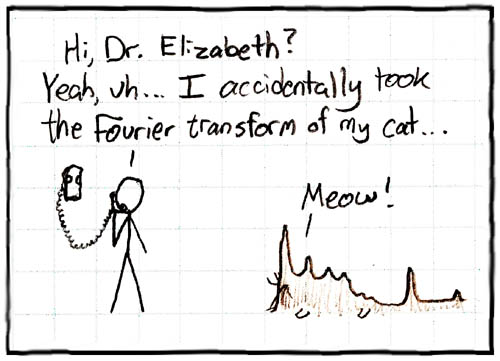
\includegraphics[height=200pt]{fourier}
\caption{Insert caption here. Image source: Randall Munroe~\cite{xkcd}. }
\label{example_figure}
\end{figure}
Figure \ref{example_figure} also gets a number automatically and will be placed where Latex thinks it looks good. You can specify a preference with h(ere), t(op), b(ottom), p(age).

\section{Equations}
Latex is also really good at printing equations: $E=mc^2$

\begin{equation}
A = \sum_{i=1}^N A_1 \cdot A_2
\end{equation}

\section{Structure}

Please structure your report in the following sections:
\begin{description}
	\item[Introduction (1 pages)] Introduce to and define the problem setting and motivate why the problem is of interest.
	\item[Method (4-6 pages)] Describe the methods you have developed and implemented.
	\item[Results (4-6 pages)] Provide qualitative and quantitative results on your approach.
	\item[Conclusions (1 page)] Summarize and discuss your approach.
\end{description}


% +++++++++++++++++++++++++

% =========================================================================
\bibliographystyle{alpha}
\bibliography{teamproject_report}

% =========================================================================

\end{document}
